\documentclass{article}
\usepackage[utf8]{inputenc}
\usepackage{amsmath}
\usepackage{amssymb}
\usepackage{amsthm}
\usepackage{float}
\usepackage[colorlinks=true]{hyperref}
\usepackage{parskip}
\usepackage{ upgreek }
\usepackage{tikz}
\usetikzlibrary{arrows,automata}
\usepackage{fancyhdr}
\usepackage{pgfplots}
\usepackage{graphicx}
\usepackage{listings}
\usetikzlibrary{intersections}
\usepackage{mathtools}

\usepackage[a4paper, total={6in, 8in}]{geometry}

\renewcommand{\vec}[1]{\mathbf{#1}}


\author{Elsie Mestl}
\date{\today}
\title{Oblig 1. \\ matinf3100- Linear optimization}


\pagestyle{fancy}
\lhead{Oblig 1. \quad matinf3100- Linear optimization}
\rhead{Elsie Mestl}

\begin{document}
\maketitle


\section*{Problem 1}
\subsection*{a)}

\begin{align*}
  \vec{x} &=
  \begin{bmatrix}
    x_1 \\
    x_2 \\
    x_3 \\
  \end{bmatrix}
  \quad
  \vec{c} =
  \begin{bmatrix}
    -7 \\
    0 \\
    2 \\
  \end{bmatrix}
  \quad
  \vec{b} =
  \begin{bmatrix}
    1 \\
    2 \\
    0 \\
  \end{bmatrix} \quad
  \mathrm{A} =
  \begin{bmatrix}
    0 && -3 && 4 \\
    1 && -1 && 0 \\
    -3 && 0 && 1 \\
  \end{bmatrix}
\end{align*}

Now the LP problem given kan be written as max$(\vec{c}^\mathrm{T}\vec{x})$ subject to $\mathrm{A}\vec{x} \leq \vec{b}$, $\vec{x} \geq \vec{0}$


\subsection*{b)}
Introduce slack variables $w_1, w_2, w_3$, and get the following dictionary.

\begin{align*}
  &\begin{matrix}
     \eta = & & - &7x_1 & & &+ &2x_3 \\
     \\
     w_1 = & 1 &  & & + &3x_2 &- &4x_3 \\
     w_2 = & 2 & -&x_1 & +&x_2 \\
     w_3 = & & & 3x_1 & & & - & x_3
   \end{matrix} \\
  &x_1, x_2, x_3, w_1, w_2, w_3 \geq 0 \\
  \intertext{Since $2x_3$ is the only variable that we can increase to make the objective value increas. This means $x_3$ is the entering variable. And by observation on the dictionary we se that $w_3$ is the leaving variable and $x_3$ can not increas at all. After change we get the following dictionary.}
  &\begin{matrix}
     \eta = & & - &x_1 & & &- &2w_3 \\
     \\
     w_1 = & 1 &  -&12x_1 & + &3x_2 &+ &4w_3 \\
     w_2 = & 2 & -&x_1 & +&x_2 \\
     x_3 = & & & 3x_1 & & & - & w_3
   \end{matrix} \\
  &x_1, x_2, x_3, w_1, w_2, w_3 \geq 0 \\
\end{align*}
Now we can not increase the objective value any more so the optimal solution is $x_1 = 0, x_2 = 0, x_3 = 0$ vith the objective value 0.

\subsection*{c)}

\begin{align*}
  \vec{x} &=
  \begin{bmatrix}
    x_1 \\
    x_2 \\
    \vdots \\
    x_n \\
    x_{n+1} \\
    \vdots \\
    x_{n+m} \\
  \end{bmatrix}
  \quad
  \vec{c} =
  \begin{bmatrix}
    c_1 \\
    c_2 \\
    \vdots \\
    c_n \\
    0 \\
    \vdots \\
    0 \\
  \end{bmatrix}
  \quad
  \vec{b} =
  \begin{bmatrix}
    b_1 \\
    b_2 \\
    \vdots \\
    b_m \\
  \end{bmatrix} \quad
  \mathrm{A'} =
  \begin{bmatrix}
    a_{11} & a_{12} & \cdots & a_{1n} \\
    a_{21} & \ddots &  & \\
    \vdots &  & \ddots &\\
    a_{m1} & a_{m2} & \cdots & a_{mn} \\
  \end{bmatrix} \\ \ \\
  \mathrm{A} &= \begin{bmatrix}
    \mathrm{A'} & \mathrm{I}_m \\
  \end{bmatrix}
\end{align*}

Now the LP problem given kan be written as max$(\vec{c}^\mathrm{T}\vec{x})$ subject to $\mathrm{A}\vec{x} = \vec{b} $, $\vec{x} \geq \vec{0}$


\section*{Problem 2}
\subsection*{a)}

Start by introducing slack variables and get the following intitial dictionary.
\begin{align*}
  &\begin{matrix}
     \eta = & & & -3x_1& + &6x_2 \\
     \\
     w_1 = & 6 & - & 2x_1& - &x_2  \\
     w_2 = & 2 & +&x_1 & -&2x_2 \\
   \end{matrix} \\
  &x_1, x_2, w_1, w_2 \geq 0 \\
  \intertext{To increas $\eta$ let $x_2$ be the entering variable and let $w_2$ be the leaving variable. Get the new dictionary.}
  &\begin{matrix}
     \eta = &6 &  && - &3w_2 \\
     \\
     x_2 = & 1 & +&\frac{x_1}{2} & -&\frac{w_2}{2} \\
     w_1 = & 5 & - & \frac{5x_1}{2}& + &\frac{w_2}{2}  \\
   \end{matrix} \\
  &x_1, x_2, w_1, w_2 \geq 0 \\
  \intertext{It is imposible to increas $\eta$, so we have reached a optimal value, $\eta = 6$. Since $x_1$ is not in the basis, but missing form the objective function this can have any value as long it doesn't contradict the restrictions. Thus all the optimal solutions are given by $w_2 = 0$ and $x_1 \leq 2$, this implies that $x_2 \in [1, 2]$.}
\end{align*}

\subsection*{b)}
\begin{figure}[H]
  \begin{minipage}[c]{7cm}
    \begin{tikzpicture}
      \draw[gray!50, thin, step=0.5] (-1,-1) grid (4,4);
      \draw[very thick,->] (-1,0) -- (4,0) node[right] {$x_2$};
      \draw[very thick,->] (0,-1) -- (0,4) node[above] {$x_1$};

      \foreach \x in {-1,...,4} \draw (\x,0.5) -- (\x,-0.5) node[below] {\tiny\x};
      \foreach \y in {-1,...,4} \draw (-0.5,\y) -- (0.5,\y) node[right] {\tiny\y};

      \foreach \x/\y/\t/\p in {0/0/A/below left,
        0/3/D/above left,
        1/0/B/bellow right,
        2/2/C/above right}
      \coordinate[label={\p:\t}] (\t) at (\x,\y);
      \fill[blue!50!cyan,opacity=0.3] (A) -- (B) -- (C) -- (D) -- cycle;

      \draw (0,3) -- node[above,sloped, near start]       {\tiny$2x_1+x_2\leq6$} (4,1);
      \draw (1,0) -- node[sloped, near start, above]       {\tiny$-x_1+2x_2\leq2$}   (3,4);
      \draw[red, thick] (1, 0) -- (2, 2)
    \end{tikzpicture}
  \end{minipage}
  \begin{minipage}[c]{\textwidth-7cm}
    The red line symbolizes alle the optimal solution. The reason there are multiple solitions is beacs the objective function is paralell to one of the restrictions.
  \end{minipage}
\end{figure}

\subsection*{c)}

Start by introducing slack variables and get the following intitial dictionary.
\begin{align*}
  &\begin{matrix}
     \eta = & & & 3x_1& + &2x_2 \\
     \\
     w_1 = & 3 & - & x_1& + &x_2  \\
     w_2 = & 2 & -&x_1 & & \\
   \end{matrix} \\
  &x_1, x_2, w_1, w_2 \geq 0 \\
  \intertext{To increas $\eta$ let $x_1$ be the entering variable and let $w_2$ be the leaving variable. Get the new dictionary.}
  &\begin{matrix}
     \eta = &6 & + & 2x_2& - &3w_2 \\
     \\
     x_1 = & 2 & & & -&w_2 \\
     w_1 = & 1 & + & x_2& + &w_2  \\
   \end{matrix} \\
  &x_1, x_2, w_1, w_2 \geq 0 \\
  \intertext{To increase $\eta$ futher let $x_2$ be the entering variable, but since we can increase $x_2$ as much as we want and still not break any restrictions we have that the problem is unbounded.}
\end{align*}


\section*{Problem 3}
\subsection*{a)}

\begin{align*}
  \text{minimize: \quad} &\sum_i|b_i - \sum_ja_{ij}x_j|\\
  \intertext{The minimalization problem above can easaly be written as the bellow by introducing $t_i = |b_i - \sum_ja_{ij}x_j|$ for $i = 1, 2, \cdots, n$:}
  \text{minimize: \quad} &\sum_i t_i \\
  \text{subject to: \quad} &t_i - |b_i - \sum_ja_{ij}x_j|  = 0, \text{\quad for $i = 1, 2, \cdots, n$}\\
  \intertext{but then $b_i - \sum_ja_{ij}x_j$ has to either be equal to $t_i$ or $-t_i$ hence we can say $b_i - \sum_ja_{ij}x_j$ lies in between the two, for all $i = 1, 2, \cdots, n$. Thus we can rewrite the prevoius to:}
  \text{minimize: \quad} &\sum_i t_i \\
  \text{subject to: \quad} &-t_i \leq b_i - \sum_ja_{ij}x_j \leq t_i, \text{\quad for $i = 1, 2, \cdots, n$}\\
\end{align*}



DETTE MÅ FIKSES!!!!!  TEKSTEN TIL SLUTT!!!!
\subsection*{b)}
\subsubsection*{Using the following code to compute $\vec{x}$ using $L_2$-regression.}
\lstinputlisting[language = Matlab, frame = single]{oblig1.m}
Here $\vec{x} = [2.1212, 0.4545]$

\newpage
\subsubsection*{Using the followin code to compute $\vec{x}$ usin $L_2$-regression.}
\lstinputlisting[language = OCL, frame = single]{Oblig1.mod}
With the given data:
\lstinputlisting[language = OCL, frame = single]{Oblig1.dat}

Here $\vec{x}= [2, 0]$

And by comparing them to the original data we get the following plot:
\begin{figure}[H]
  \centering
  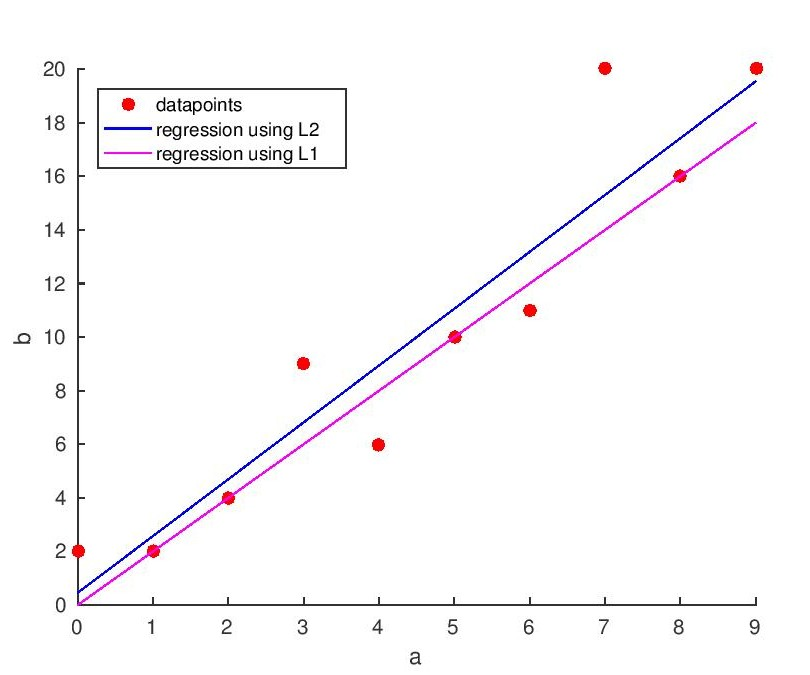
\includegraphics[scale = 0.3]{plot.jpg}
\end{figure}

Yes, the difference is as expected. The $L_2$ doesn't hit any of the data points but lies more in the middel, where as the $L_1$ regression hist 4 points but then som of the outliners become quite far of.

I suppose depending on what kind of data-set one has they have both their preferences. As said above the $L_1$ regression, using the simplex method, does not care about abnormalities in such extent as $L_2$ so if there is not a lot of data I would say $L_1$ is to prefer.



\end{document}
